\documentclass[12pt]{article}
\usepackage{graphicx}
\usepackage{tikz}
\usepackage{aeguill}

\begin{document}
\begin{titlepage}
  \begin{center}
    \large{University of Puerto Rico\\
    Mayagüez Campus\\
    \vspace{\baselineskip}
    Department of Electrical and Computer Engineering}
  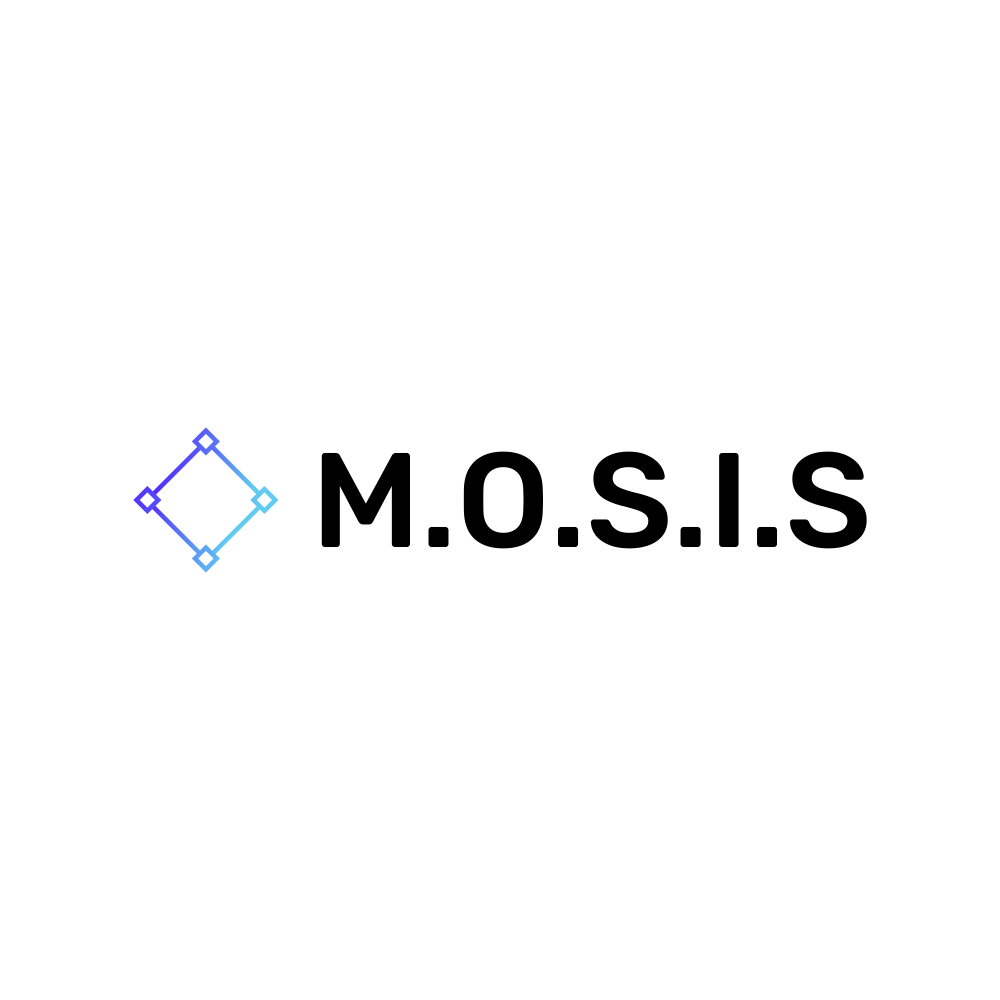
\includegraphics[scale=0.2]{../Title_Page/default.png}\\
    \Huge{\underline{M.O.S.I.S Host Software}\\}
    \Huge{\underline{User Guide}\\}
    \vspace{5cm}
    \large by\\
    Fabio J. Matos Nieves\\
    \normalsize
  \end{center}
\end{titlepage}

\tableofcontents
\listoffigures
\newpage
\section{Introduction}
The M.O.S.I.S microscope captures \textit{in situ} metadata and stereoscopic images for marine specimens. This tool is invaluable to study marine life in a wildlife setting where the conditions in the lab cannot be replicated accurately. It stores the captured media on its on board solid state memory along. This arrangement raises the following question: ``How will the data be viewed by a researcher after capture''. One answer to that question would be to review the data on the microscope itself and in a perfect world this would be the most straightforward solution. But alas, we do not live in a perfect world and reviewing the data on the microscope itself would be inadvisable for the following reasons:
\begin{itemize}
\item What if the microscope gets damaged during use in the field?
\item Would a researcher know how to retrieve/export the data captured by this device?
\end{itemize}
To answer the first question, in the best case scenario, the data would be temporarily insensible until repairs are completed. In the worst case, the data would be permanently lost due to the device being irreparably damaged. This leads to the second question where even if the solid state drive is still functioning in the case of hardware failure of the microscope, the data would require somebody experienced enough with the architecture of the device and the operating system that it runs on in order to retrieve the data safely. In addition, with the current arrangement, there is one, and only one copy of the data, meaning if the solid state drive fails, all of the data is gone. Finally, the microscope needs to be configured for the type of study being done before hand by a researcher. Given that the microscope only has 8 buttons and a 4 inch display, configuring the type of study on the device would be extremely cumbersome not just on land but even more so in the field. Thus, a piece of software is needed that addresses all of these concerns, in a package that a researcher can easily use, which we will call the ``Host Software''.
\section{What will the host software do?}
The host software will need to accomplish at a minimum 3 tasks:
\begin{enumerate}
\item Enforce and streamline the process of backing up the data captured by the microscope and to backup the microscope's operating system.
\item Display the data captured by the M.O.S.I.S microscope and do simple analysis on the data.
  \item Configure the type of study to be performed on the microscope remotely.
\end{enumerate}
\section{What are the client requirements for the host software?}
\subsection{Domain Requirements}
\begin{itemize}
	\item The system-to-be must allow the backup of the M.O.S.I.S project Raspberry Pi's operating system.
	\item The system-to-be must allow the backup of the images captured by the M.O.S.I.S project Raspberry Pi.
	\item The system-to-be must have a database that stores the media captured by the M.O.S.I.S project Raspberry Pi.
	\item The system-to-be must have a database that stores the sensor captured by the M.O.S.I.S project Raspberry Pi.
	\item The system-to-be must create a stereoscopic image from the media captured by the M.O.S.I.S project Raspberry Pi.
	\item The system-to-be must have the means to pre-configured the type of media capture before and after deployment in the field.
	\item The system-to-be must tag the media captured the M.O.S.I.S Raspberry Pi with the information stored in the database.
	\item The system-to-be must analyze the captured media for bleaching estimates.
	\item The system-to-be must analyze the captured media for area coverage by color.
\end{itemize}
\subsection{Interface Requirements}
\begin{itemize}
	\item The system-to-be's database must contain image information that includes:
	      \begin{itemize}
		      \item Left Camera Image
		      \item Right Camera Image
		      \item Time Stamp
		      \item Temperature
		      \item Ph
		      \item Pressure
		      \item Dissolved Oxygen (DO) Content
	      \end{itemize}
	\item The system-to-be must have a home page where there is a preview of all images currently within the database.
	\item The system-to-be must create an individual page for each entry within the database.
\end{itemize}
\section{What channels of communication are involved for the host software to function?}
There two main communication channels: ``microscope to host computer'', ``host computer to microscope'' and ``host computer and host computer web browser''. The main reason why the microscope will communicate to the host computer, i.e the computer running the host software, will be to send a copy of all of the data stored on the solid state drive to the host computer in order to have a backup of the data. Vice versa, the host computer will communicate with the microscope to send the studies to be performed on the microscope. Lastly, the host computer will communicate to a web browser the local website where the analyzed data will be presented and where the microscope can be configured from.
\section{UML Diagrams}
\begin{figure}[h!]
	% generated by Plantuml 1.2023.10      
	\definecolor{plantucolor0000}{RGB}{24,24,24}
	\definecolor{plantucolor0001}{RGB}{0,0,0}
	\definecolor{plantucolor0002}{RGB}{241,241,241}
	\resizebox{\textwidth}{!}{
		\begin{tikzpicture}[yscale=-1
				,pstyle0/.style={color=plantucolor0000,line width=1.0pt}
				,pstyle1/.style={color=plantucolor0000,fill=plantucolor0002,line width=0.5pt}
				,pstyle2/.style={color=plantucolor0000,fill=plantucolor0002,line width=1.5pt}
				,pstyle3/.style={color=plantucolor0000,fill=plantucolor0000,line width=1.0pt}
			]
			\draw[pstyle0] (105.5pt,12pt) arc (180:270:5pt) -- (110.5pt,7pt) -- (742.5pt,7pt) arc (270:360:5pt) -- (747.5pt,12pt) -- (747.5pt,541pt) arc (0:90:5pt) -- (742.5pt,546pt) -- (110.5pt,546pt) arc (90:180:5pt) -- (105.5pt,541pt) -- cycle;
			\node at (368.2762pt,9pt)[below right,color=black]{\textbf{Host-Software}};
			\draw[pstyle1] (230.0396pt,64.2079pt) ellipse (81.5396pt and 18.7079pt);
			\node at (173.1751pt,53.975pt)[below right,color=black]{Download RPi};
			\draw[pstyle1] (229.8321pt,137.9664pt) ellipse (87.8321pt and 19.9664pt);
			\node at (164.5513pt,127.7334pt)[below right,color=black]{Configure Study};
			\draw[pstyle1] (230.2208pt,211.9442pt) ellipse (80.2208pt and 18.4442pt);
			\node at (175.1922pt,201.7112pt)[below right,color=black]{Upload Study};
			\draw[pstyle1] (229.8715pt,287.0743pt) ellipse (93.3715pt and 21.0743pt);
			\node at (157.5382pt,276.8413pt)[below right,color=black]{Preview All Media};
			\draw[pstyle1] (565.1453pt,70.0291pt) ellipse (110.6453pt and 24.5291pt);
			\node at (472.1259pt,59.7961pt)[below right,color=black]{Export Selected Entries};
			\draw[pstyle1] (230.166pt,367.1332pt) ellipse (108.666pt and 24.1332pt);
			\node at (139.4444pt,356.9002pt)[below right,color=black]{Examine Specific entry};
			\draw[pstyle1] (564.7769pt,247.1554pt) ellipse (166.2769pt and 35.6554pt);
			\node at (414.6137pt,235.6214pt)[below right,color=black]{View Automatically Generated Analysis};
			\draw[pstyle1] (564.9344pt,153.1869pt) ellipse (103.9344pt and 23.1869pt);
			\node at (479.7707pt,142.9539pt)[below right,color=black]{Export Specific Entry};
			\draw[pstyle1] (229.8504pt,444.1701pt) ellipse (78.8504pt and 18.1701pt);
			\node at (176.762pt,433.9371pt)[below right,color=black]{Filter Entries};
			\draw[pstyle1] (565.2264pt,507.0453pt) ellipse (103.2264pt and 23.0453pt);
			\node at (480.903pt,496.8123pt)[below right,color=black]{Filter Entries by Date};
			\draw[pstyle1] (564.8649pt,427.073pt) ellipse (95.8649pt and 21.573pt);
			\node at (489.4395pt,416.84pt)[below right,color=black]{Filter Entries by ID};
			\draw[pstyle1] (565.0426pt,344.2085pt) ellipse (121.5426pt and 26.7085pt);
			\node at (460.5931pt,333.5986pt)[below right,color=black]{Filter Entries by Shot Type};
			\draw[pstyle2] (33pt,226.5pt) ellipse (16pt and 16pt);
			\draw[pstyle2] (33pt,246.5pt) ..controls (37pt,246.5pt) and (40pt,246.5pt) .. (44pt,242.5pt) ..controls (52pt,242.5pt) and (60pt,250.5pt) .. (60pt,258.5pt) -- (60pt,262.5pt) ..controls (60pt,266.5pt) and (56pt,270.5pt) .. (52pt,270.5pt) -- (14pt,270.5pt) ..controls (10pt,270.5pt) and (6pt,266.5pt) .. (6pt,262.5pt) -- (6pt,258.5pt) ..controls (6pt,250.5pt) and (14pt,242.5pt) .. (22pt,242.5pt) ..controls (26pt,246.5pt) and (29pt,246.5pt) .. (33pt,246.5pt);
			\node at (15.6667pt,272pt)[below right,color=black]{User};
			\draw[pstyle0] (41.14pt,208.85pt) ..controls (49.15pt,174.94pt) and (65.47pt,128.02pt) .. (97.5pt,100pt) ..controls (112.53pt,86.85pt) and (131.93pt,78.46pt) .. (151.19pt,73.12pt);
			\draw[pstyle3] (156.08pt,71.83pt) -- (146.3593pt,70.2465pt) -- (151.2439pt,73.0997pt) -- (148.3907pt,77.9843pt) -- (156.08pt,71.83pt) -- cycle;
			\draw[pstyle0] (61.71pt,209.33pt) ..controls (71.74pt,197.13pt) and (83.97pt,184.7pt) .. (97.5pt,176pt) ..controls (114.64pt,164.98pt) and (135.04pt,157.08pt) .. (154.61pt,151.45pt);
			\draw[pstyle3] (159.56pt,150.06pt) -- (149.8162pt,148.6252pt) -- (154.7438pt,151.4034pt) -- (151.9656pt,156.331pt) -- (159.56pt,150.06pt) -- cycle;
			\draw[pstyle0] (61.53pt,244.64pt) ..controls (87.84pt,239.51pt) and (128.53pt,231.58pt) .. (163.22pt,224.82pt);
			\draw[pstyle3] (168.29pt,223.83pt) -- (158.6913pt,221.6244pt) -- (163.3822pt,224.7859pt) -- (160.2207pt,229.4768pt) -- (168.29pt,223.83pt) -- cycle;
			\draw[pstyle0] (61.53pt,255.22pt) ..controls (85.24pt,259.72pt) and (120.64pt,266.44pt) .. (152.78pt,272.54pt);
			\draw[pstyle3] (157.91pt,273.51pt) -- (149.8249pt,267.8858pt) -- (152.9996pt,272.5679pt) -- (148.3175pt,275.7425pt) -- (157.91pt,273.51pt) -- cycle;
			\draw[pstyle0] (61.76pt,291pt) ..controls (71.8pt,303.35pt) and (84.02pt,316pt) .. (97.5pt,325pt) ..controls (112.44pt,334.97pt) and (129.9pt,342.71pt) .. (147.13pt,348.66pt);
			\draw[pstyle3] (151.98pt,350.29pt) -- (144.7128pt,343.6426pt) -- (147.238pt,348.7046pt) -- (142.1761pt,351.2298pt) -- (151.98pt,350.29pt) -- cycle;
			\draw[pstyle0] (40.09pt,291.18pt) ..controls (47.54pt,327.02pt) and (63.62pt,377.81pt) .. (97.5pt,408pt) ..controls (112.81pt,421.65pt) and (132.83pt,430.18pt) .. (152.6pt,435.5pt);
			\draw[pstyle3] (157.62pt,436.78pt) -- (149.8799pt,430.6897pt) -- (152.7735pt,435.5505pt) -- (147.9127pt,438.4441pt) -- (157.62pt,436.78pt) -- cycle;
			\draw[pstyle0] (315.89pt,263.9pt) ..controls (324.1pt,259.48pt) and (331.83pt,254.23pt) .. (338.5pt,248pt) ..controls (386.76pt,202.89pt) and (348.05pt,154.66pt) .. (398.5pt,112pt) ..controls (416.95pt,96.4pt) and (440.42pt,86.48pt) .. (463.86pt,80.2pt);
			\draw[pstyle0] (318.5pt,270.41pt) -- (297.39pt,272.32pt) -- (312.7pt,257.66pt) -- (318.5pt,270.41pt) -- cycle;
			\draw[pstyle0] (303.58pt,338.9pt) ..controls (315.28pt,334.3pt) and (327.23pt,329.55pt) .. (338.5pt,325pt) ..controls (365.29pt,314.19pt) and (371.39pt,309.97pt) .. (398.5pt,300pt) ..controls (421.01pt,291.72pt) and (445.5pt,283.47pt) .. (468.57pt,276.04pt);
			\draw[pstyle0] (306.13pt,345.42pt) -- (284.95pt,346.19pt) -- (301.03pt,332.38pt) -- (306.13pt,345.42pt) -- cycle;
			\draw[pstyle0] (319.04pt,339.49pt) ..controls (326.07pt,335.29pt) and (332.68pt,330.49pt) .. (338.5pt,325pt) ..controls (385.05pt,281.03pt) and (349.2pt,234.87pt) .. (398.5pt,194pt) ..controls (418.21pt,177.66pt) and (443.5pt,167.68pt) .. (468.34pt,161.63pt);
			\draw[pstyle0] (321.96pt,345.86pt) -- (300.96pt,348.69pt) -- (315.61pt,333.38pt) -- (321.96pt,345.86pt) -- cycle;
			\draw[pstyle0] (311.13pt,459.16pt) ..controls (364.15pt,469.19pt) and (433.33pt,482.28pt) .. (485.92pt,492.23pt);
			\draw[pstyle0] (309.65pt,466pt) -- (291.3pt,455.41pt) -- (312.26pt,452.25pt) -- (309.65pt,466pt) -- cycle;
			\draw[pstyle0] (327.55pt,439.07pt) ..controls (372.84pt,436.76pt) and (426.56pt,434.02pt) .. (471.35pt,431.73pt);
			\draw[pstyle0] (327.73pt,446.07pt) -- (307.4pt,440.1pt) -- (327.01pt,432.09pt) -- (327.73pt,446.07pt) -- cycle;
			\draw[pstyle0] (294.36pt,422.79pt) ..controls (341.22pt,407.11pt) and (397.14pt,388.41pt) .. (398.5pt,388pt) ..controls (426.41pt,379.63pt) and (457.2pt,371.22pt) .. (484.58pt,364.03pt);
			\draw[pstyle0] (296.54pt,429.44pt) -- (275.35pt,429.15pt) -- (292.09pt,416.17pt) -- (296.54pt,429.44pt) -- cycle;
		\end{tikzpicture}
	}
	\caption{M.O.S.I.S Host Software UseCase Diagram}
\end{figure}

\newpage
% generated by Plantuml 1.2023.10      
\definecolor{plantucolor0000}{RGB}{241,241,241}
\definecolor{plantucolor0001}{RGB}{24,24,24}
\definecolor{plantucolor0002}{RGB}{0,0,0}
\begin{figure}
\begin{tikzpicture}[yscale=-1
,pstyle0/.style={color=plantucolor0001,fill=plantucolor0000,line width=0.5pt}
,pstyle1/.style={color=plantucolor0001,line width=1.0pt}
,pstyle2/.style={color=plantucolor0001,fill=plantucolor0001,line width=1.0pt}
]
\draw[pstyle0] (87pt,12pt) arc (180:270:5pt) -- (92pt,7pt) -- (210.9714pt,7pt) arc (270:360:5pt) -- (215.9714pt,12pt) -- (215.9714pt,51.0679pt) arc (0:90:5pt) -- (210.9714pt,56.0679pt) -- (92pt,56.0679pt) arc (90:180:5pt) -- (87pt,51.0679pt) -- cycle;
\draw[pstyle0] (195.9714pt,12pt) rectangle (210.9714pt,22pt);
\draw[pstyle0] (193.9714pt,14pt) rectangle (197.9714pt,16pt);
\draw[pstyle0] (193.9714pt,18pt) rectangle (197.9714pt,20pt);
\node at (102pt,27pt)[below right,color=black]{Rasberry Pi};
\draw[pstyle0] (7pt,199pt) arc (180:270:5pt) -- (12pt,194pt) -- (159.3188pt,194pt) arc (270:360:5pt) -- (164.3188pt,199pt) -- (164.3188pt,238.0679pt) arc (0:90:5pt) -- (159.3188pt,243.0679pt) -- (12pt,243.0679pt) arc (90:180:5pt) -- (7pt,238.0679pt) -- cycle;
\draw[pstyle0] (144.3188pt,199pt) rectangle (159.3188pt,209pt);
\draw[pstyle0] (142.3188pt,201pt) rectangle (146.3188pt,203pt);
\draw[pstyle0] (142.3188pt,205pt) rectangle (146.3188pt,207pt);
\node at (22pt,214pt)[below right,color=black]{Host Computer};
\draw[pstyle0] (78.5pt,386pt) arc (180:270:5pt) -- (83.5pt,381pt) -- (219.2714pt,381pt) arc (270:360:5pt) -- (224.2714pt,386pt) -- (224.2714pt,425.0679pt) arc (0:90:5pt) -- (219.2714pt,430.0679pt) -- (83.5pt,430.0679pt) arc (90:180:5pt) -- (78.5pt,425.0679pt) -- cycle;
\draw[pstyle0] (204.2714pt,386pt) rectangle (219.2714pt,396pt);
\draw[pstyle0] (202.2714pt,388pt) rectangle (206.2714pt,390pt);
\draw[pstyle0] (202.2714pt,392pt) rectangle (206.2714pt,394pt);
\node at (93.5pt,401pt)[below right,color=black]{Web Browser};
\draw[pstyle0] (151.5pt,125pt) ellipse (8pt and 8pt);
\node at (136.1889pt,142pt)[below right,color=black]{SSH};
\draw[pstyle0] (151.5pt,312pt) ellipse (8pt and 8pt);
\node at (105.7709pt,329pt)[below right,color=black]{Web Server};
\draw[pstyle1] (140.19pt,56.06pt) ..controls (137.72pt,73.61pt) and (138.43pt,96.89pt) .. (142.31pt,111.14pt);
\draw[pstyle2] (143.89pt,115.96pt) -- (144.8918pt,106.1622pt) -- (142.3346pt,111.2081pt) -- (137.2887pt,108.6509pt) -- (143.89pt,115.96pt) -- cycle;
\draw[pstyle1] (159.56pt,115.96pt) ..controls (164.63pt,103.84pt) and (166.16pt,80.29pt) .. (164.14pt,61.29pt);
\draw[pstyle2] (163.48pt,56.06pt) -- (160.6439pt,65.4917pt) -- (164.109pt,61.0203pt) -- (168.5804pt,64.4853pt) -- (163.48pt,56.06pt) -- cycle;
\draw[pstyle1] (145.64pt,134.12pt) ..controls (136.73pt,146.48pt) and (119.33pt,170.6pt) .. (105.53pt,189.73pt);
\draw[pstyle2] (102.46pt,193.98pt) -- (110.9709pt,189.0237pt) -- (105.3864pt,189.9259pt) -- (104.4842pt,184.3414pt) -- (102.46pt,193.98pt) -- cycle;
\draw[pstyle1] (102.5pt,243.06pt) ..controls (115.37pt,260.91pt) and (132.54pt,284.71pt) .. (142.76pt,298.89pt);
\draw[pstyle2] (145.7pt,302.96pt) -- (143.6758pt,293.3214pt) -- (142.7736pt,298.9059pt) -- (137.1891pt,298.0037pt) -- (145.7pt,302.96pt) -- cycle;
\draw[pstyle1] (143.86pt,321.12pt) ..controls (139.09pt,333.27pt) and (137.66pt,356.79pt) .. (139.57pt,375.76pt);
\draw[pstyle2] (140.2pt,380.98pt) -- (143.0928pt,371.5656pt) -- (139.6009pt,376.016pt) -- (135.1504pt,372.5241pt) -- (140.2pt,380.98pt) -- cycle;
\draw[pstyle1] (163.47pt,380.98pt) ..controls (166.09pt,363.47pt) and (165.35pt,340.21pt) .. (161.25pt,325.94pt);
\draw[pstyle2] (159.59pt,321.12pt) -- (158.7388pt,330.932pt) -- (161.2182pt,325.8475pt) -- (166.3027pt,328.3269pt) -- (159.59pt,321.12pt) -- cycle;
\draw[pstyle1] (156.36pt,303pt) ..controls (163.54pt,290.65pt) and (176.66pt,265.98pt) .. (181.5pt,243pt) ..controls (185.99pt,221.69pt) and (185.99pt,215.31pt) .. (181.5pt,194pt) ..controls (177.19pt,173.53pt) and (166.31pt,151.72pt) .. (158.91pt,138.48pt);
\draw[pstyle2] (156.36pt,134pt) -- (157.3349pt,143.8005pt) -- (158.833pt,138.3456pt) -- (164.2879pt,139.8437pt) -- (156.36pt,134pt) -- cycle;
\end{tikzpicture}
\caption{Host Software Communication Diagram}  
\label{figure:Host-Software-Communication-Diagram}
\end{figure}

\end{document}
%%% Local Variables:
%%% mode: latex
%%% TeX-master: t
%%% End:
